% Printed 242; principal PDF 249; Google PDF 253.
\par\clearpage
\noindent\makebox[0pt][l]{\fontsize{13}{16}\selectfont 242}\hfill{\small\textbf{BEMERKUNGEN.\quad TRIGONOMETRISCHE PUNKTBESTIMMUNG.}}\hfill\null\par\medskip

{\small
\noindent Punkte geschnitten werden könnten. Es genügt, von diesen Punkten aus andere Punkte einzuschneiden, die bereits festgelegt sind. Es müssen jedoch mindestens 3 sein. Hat man 4 geschnitten, so hat man eine Kontrolle. Stimmen diese 4 jedoch nicht überein, was ebenfalls nicht selten ist, da es leicht zu einer Verwechslung kommen kann, so weiß man nicht, wo der Fehler liegt. Deshalb ist es besser, 5 oder mehr einzuschneiden. . . . . Überhaupt kann man nicht nachdrücklich genug empfehlen, jeden Punkt so oft wie irgend möglich einzuschneiden, selbst wenn man die Schnitte nicht nach der Methode der kleinsten Quadrate vereinigen will. Auf diese Weise ist man vor Fehlern geschützt, und auch ein Punkt, der weder Haupt- noch Nebenpunkt ist, kann, sobald er genau bestimmt ist, häufig dazu dienen, die Identität eines anderen Punkts festzustellen. Hat man nun auch für die Nebenpunkte die Koordinaten berechnet, so geht man zur Bestimmung der übrigen eingeschnittenen Punkte über. \textsc{Gauss} führt darüber, nachdem alle\\
\makebox[0pt][r]{.\enspace}Rechnungen abgeschlossen sind, das folgende Protokoll.
\[
 \overbrace{\text{\textls[120]{Krückeberg}}}^{A}
 \quad\overbrace{-71364{,}939\qquad+45842{,}386}^{B}
\]
\[
\begin{array}{@{}l@{\qquad}r@{\qquad}r@{\qquad}r@{\;}r@{\;}r@{\qquad}r@{}}
 \multicolumn{1}{c}{a}&\multicolumn{1}{c}{b}&\multicolumn{1}{c}{c}&
 \multicolumn{3}{c}{d}&\multicolumn{1}{c@{}}{e}\\
 \text{Süntel}&-70637{,}258&+37481{,}447&94^\circ&58'&27''{,}964&-0{,}885\\
 \text{Klütberg}&-63179{,}059&+41387{,}660&151&26&44{,}009&-1{,}553\\
 \text{Wittekindstein}&-80356{,}285&+71875{,}835&289&3&13{,}703&-0{,}329\\
 \text{Pagenburg}&-75427{,}470&+50454{,}707&311&22&31{,}882&+0{,}448\\
 \hline
 \multicolumn{7}{c@{}}{\text{\textls[120]{Sachsenhagen, Schloss}}\;-96486{,}713\qquad+46075{,}741}\\
 \text{Wittekindstein}&-80356{,}285&+71875{,}835&237&59&11{,}516&\\
 \text{Bergkirchen}&-99061{,}252&+47440{,}144&332&4&3{,}954.&\\
 \hline
\end{array}
\]

\(A\) ist der Ort, dessen Koordinaten bestimmt werden. Diese Koordinaten sind unter \(B\) angegeben. Unter \(a\) stehen die Namen der Orte, von denen aus \(A\) bestimmt wurde, unter \(b,c\) ihre Koordinaten, unter \(d\) das beobachtete Azimut und unter \(e\) die Differenz zwischen dem aus den Koordinaten berechneten und dem beobachteten Azimut. Diese Spalte fällt also weg, wenn wir \textls[120]{nicht mehr} Daten haben, als zur Bestimmung des fraglichen Punkts nötig sind. Die einzelnen in diesem Protokoll erfassten Punkte werden nicht eigens geordnet. Man lässt jedoch am besten etwas Platz frei, um spätere Bemerkungen und Schnitte, die man erst nach der Berechnung und Eintragung gefunden hat, nachzutragen. Im Übrigen trägt man die Punkte in der Reihenfolge in dieses Protokoll ein, in der man sie berechnet hat. In den Tabellen markiert man die Schnitte, die bereits für die Berechnung verwendet wurden, damit man leichter sieht, welche Schnitte noch nicht bearbeitet sind.«

Im Nachlass ist noch eine große Anzahl solcher Protokolle vorhanden. Im Arbeitsbericht für 1844 sagt \textsc{Gauss}: »Die Ergebnisse [Koordinaten] wurden jedes Jahr nach der Verarbeitung der Messungen in Verzeichnisse eingetragen. Es sind sechzehn solcher Teilverzeichnisse vorhanden, die zusammen etwas über 3000 Bestimmungen enthalten. Die Anzahl der Punkte selbst dürfte jedoch um etwa ein Siebtel geringer sein, da viele Punkte, die in einem späteren Jahr nach dem Hinzukommen neuer Daten genauer oder zuverlässiger bestimmt werden konnten, in mehr als einem Verzeichnis auftreten. . . . . Für größere Sicherheit und bequemere Nutzung habe ich jetzt begonnen, die Teilverzeichnisse in einem einzigen zusammenzuführen, das demnach etwa 2600 Punkte enthalten wird.« (Band IV, S. 413).

In Art. 6 des Abdrucks der aus den Astr. Nachr. übernommenen Abhandlung wurden mehrere Druck- und Rechenfehler berichtigt.\hfill\textsc{Krüger.}\par
\begin{center}\rule{4cm}{.4pt}\end{center}
}

% Printed 243; principal PDF 250; Google PDF 254.
\par\clearpage

\thispagestyle{empty}
\vspace*{.23\textheight}
{\centering
{\LARGE AUSGLEICHUNG\par}
\medskip
{\LARGE\bfseries EINFACHER FIGUREN.\par}
}
\vfill
\noindent\hfill31\textsuperscript{*}\hspace*{.15\linewidth}\par
\vspace*{.14\textheight}

% Printed 244; principal PDF 251; Google PDF 255.
\par\clearpage

\null\thispagestyle{empty}

% Printed 245; principal PDF 252; Google PDF 256.
\par\clearpage

\thispagestyle{empty}
\vspace*{3\baselineskip}
{\centering\Large\bfseries NACHLASS UND BRIEFWECHSEL.\par}
\vspace{3\baselineskip}
{\centering
[1.]\par\smallskip
Ausgleichung eines Vierecks.\par}
\begin{flushleft}
\hspace*{1.8em}\(0,1,2,3\) . . . die vier Punkte\\
\hspace*{1.8em}\(01\) . . . . . . . . sowohl Länge als Richtung der Linie \(01\)\\
\hspace*{1.8em}\(C^{01}\) usw. sind Ausgleichungen, durch die alles miteinander vereinbar wird,
\end{flushleft}
\[
 C^{01}=\left[\tfrac12(C^{01}+C^{10})+\tfrac12(C^{01}-C^{10})=\right]S^{01}+D^{01},
\]
\noindent wo
\[
 S^{01}=S^{10},\qquad D^{01}=-D^{10};
\]
{\centering usw.\par}

[Man setze]
\[
 \log\operatorname{hyp}
 \frac{\sin(30-31)\sin(10-12)\sin(20-23)}
      {\sin(32-30)\sin(13-10)\sin(21-20)}
 =\lambda^0
\]
\[
\begin{array}{@{}r@{\;=\;}l@{}}
 12\,.\,13\,.\sin(12-13)&T^0\\
 02\,.\,03\,.\sin(03-02)&T'\\
 03\,.\,13\,.\sin(30-31)&T''\\
 02\,.\,12\,.\sin(21-20)&T'''.
\end{array}
\]

Hier bezeichnen \(T^0,T',T'',T'''\) die doppelten Flächeninhalte der vier Dreiecke. Man beachte, dass immer zwei Vertauschungen zugleich vorgenommen werden müssen. So entsteht \(T'\) aus \(T^0\), wenn man \(0\) mit \(1\) und \(2\) mit \(3\) vertauscht. Es gilt [da \(T^0\) und \(T''\) das entgegengesetzte Vorzeichen von \(T'\) und \(T'''\) haben]
\[
 0=T^0+T'+T''+T'''.
\]
Ebenso entstehen \(\lambda',\lambda'',\lambda'''\) aus \(\lambda^0\).

% Printed 246; principal PDF 253; Google PDF 257.
\par\clearpage
\noindent\makebox[0pt][l]{\fontsize{13}{16}\selectfont 246}\hfill{\small\textbf{NACHLASS.}}\hfill\null\par\medskip

Man hat dann
\[
\resizebox{\linewidth}{!}{\(\begin{aligned}
 {[}0={}&\lambda^0+\frac{\sin(13-12)}{\sin(10-12)\sin(13-10)}C^{10}
 -\operatorname{cotang}(10-12)\,.\,C^{12}
 -\operatorname{cotang}(13-10)\,.\,C^{13}\\
 &+\frac{\sin(21-23)}{\sin(20-23)\sin(21-20)}C^{20}
 -\operatorname{cotang}(21-20)\,.\,C^{21}
 -\operatorname{cotang}(20-23)\,.\,C^{23}\\
 &+\frac{\sin(32-31)}{\sin(30-31)\sin(32-30)}C^{30}
 -\operatorname{cotang}(30-31)\,.\,C^{31}
 -\operatorname{cotang}(32-30)\,.\,C^{32}
\end{aligned}\)}
\]
\noindent oder
\[
\begin{aligned}
 0={}&\lambda^0-\frac{01^2\,.\,T^0}{T''T'''}C^{10}
 -\tfrac12\frac{01^2+12^2-02^2}{T'''}C^{12}
 -\tfrac12\frac{01^2+13^2-03^2}{T''}C^{13}\\
 &-\frac{02^2\,.\,T^0}{T'T'''}C^{20}
 -\tfrac12\frac{02^2+12^2-01^2}{T'''}C^{21}
 -\tfrac12\frac{02^2+23^2-03^2}{T'}C^{23}\\
 &-\frac{03^2\,.\,T^0}{T'T''}C^{30}
 -\tfrac12\frac{03^2+13^2-01^2}{T''}C^{31}
 -\tfrac12\frac{03^2+23^2-02^2}{T'}C^{32}
\end{aligned}
\]
\noindent oder]
\[
\begin{array}{@{}r@{\;}r@{\;}l@{}}
 -T'T''T'''\lambda^0={}&-T^0T'\,.\,01^2\,.\,S^{01}&+T^0T'\,.\,01^2\,.\,D^{01}\\
 &-T^0T''\,.\,02^2\,.\,S^{02}&+T^0T''\,.\,02^2\,.\,D^{02}\\
 &-T^0T'''\,.\,03^2\,.\,S^{03}&+T^0T'''\,.\,03^2\,.\,D^{03}\\
 &-T'T'''\,.\,13^2\,.\,S^{13}&+T'T'''\,.\,(03^2-01^2)D^{13}\\
 &-T'T''\,.\,12^2\,.\,S^{21}&+T'T''\,.\,(01^2-02^2)D^{21}\\
 &-T''T'''\,.\,23^2\,.\,S^{32}&+T''T'''\,.\,(02^2-03^2)D^{32}\\
 =&\Sigma^0&+\qquad\Delta^0.
\end{array}
\]

\(\Sigma',\Sigma'',\Sigma'''\) sind identisch gleich \(\Sigma^0\). \(\lambda^0,\lambda',\lambda'',\lambda'''\) sind proportional zu \(T^0,T',T'',T'''\), wenn die Winkelsummen schon ausgeglichen sind. Dagegen müssen \(\Delta',\Delta'',\Delta'''\) zahlenmäßig gleich \(\Delta^0\) werden, wenn diese Ausgleichung beibehalten wird. In symmetrischer Form lautet dieser Wert
\[
\begin{aligned}
 \tfrac14(\Delta^0+\Delta'+\Delta''+\Delta''')=\tfrac14\bigl\{&
 T^0T'D^{01}(12^2+13^2-02^2-03^2)\\
 &+T^0T''D^{02}(12^2+23^2-01^2-03^2)\\
 &+T^0T'''D^{03}(13^2+23^2-01^2-02^2)\\
 &+T'T'''D^{13}(03^2+23^2-01^2-12^2)\\
 &+T'T''D^{21}(01^2+13^2-02^2-23^2)\\
 &+T''T'''D^{32}(02^2+12^2-03^2-13^2)\bigr\}.
\end{aligned}
\]

Jeden Ausdruck \(\Delta=H^{01}D^{01}+H^{02}D^{02}+\cdots\) bringt man in die Form, in der die Summe der Quadrate der Koeffizienten minimal wird, indem man

% Printed 247; principal PDF 254; Google PDF 258.
\par\clearpage
\noindent\null\hfill{\small\textbf{AUSGLEICHUNG EINFACHER FIGUREN.}}\hfill\makebox[0pt][r]{\fontsize{13}{16}\selectfont 247}\par\medskip

\noindent schreibt
\[
\begin{array}{@{}l@{\;}l@{\;}l@{}}
 \text{anstatt}&
 H^{01}\,.\,.\,.\,.\,.\,.\,.\,.&
 \tfrac14(2H^{01}-H^{20}-H^{30}+H^{21}+H^{31})\\
 \text{\quad»}&
 H^{02}\,.\,.\,.\,.\,.\,.\,.\,.&
 \tfrac14(2H^{02}-H^{10}-H^{30}+H^{12}+H^{32})\\
 \multicolumn{3}{c@{}}{\text{usw.,}}
\end{array}
\]
\noindent wo \(H^{\alpha\beta}=-H^{\beta\alpha}\).

[Addiert man nämlich zum Ausdruck für \(\Delta^0\) die 3 Winkelgleichungen, die \(T',T'',T'''\) entsprechen und bereits ausgeglichen sein sollen, nachdem man sie mit den Faktoren \(\tfrac12\mu_1,\tfrac12\mu_2,\tfrac12\mu_3\) multipliziert hat, so ändert sich \(\Delta^0\) nicht. (Die Konstante \(\lambda^0\) muss natürlich jetzt auch mit den Werten berechnet sein, die sich aus der Ausgleichung der Winkelgleichungen ergeben haben). Daher gilt auch, da die Winkelgleichungen nun lauten
\[
 \resizebox{\linewidth}{!}{\(0=-C^{02}+C^{03}-C^{23}+C^{20}-C^{30}+C^{32}
 =2(-D^{02}+D^{03}+D^{32}),\ \text{usw.:}\)}
\]
\[
\begin{aligned}
 \Delta^0={}&H^{01}D^{01}+H^{02}D^{02}+H^{03}D^{03}
             +H^{13}D^{13}+H^{21}D^{21}+H^{32}D^{32}\\
 &+\mu_1(-D^{02}+D^{03}+D^{32})+\mu_2(-D^{01}+D^{03}-D^{13})\\
 &\hspace{3.3em}+\mu_3(-D^{01}+D^{02}+D^{21}).
\end{aligned}
\]

Bestimmt man nun \(\mu_1,\mu_2,\mu_3\) so, dass die Summe der Quadrate der Koeffizienten von \(D^{01},D^{02}\) usw. minimal wird, so erhält man
\[
\begin{array}{@{}r@{\;}r@{\;}r@{\;=\;}l@{}}
 3\mu_1&+\mu_2&-\mu_3&H^{02}-H^{03}-H^{32}\\
 \mu_1&+3\mu_2&+\mu_3&H^{01}-H^{03}+H^{13}\\
 -\mu_1&+\mu_2&+3\mu_3&H^{01}-H^{02}-H^{21},
\end{array}
\]
\noindent also
\[
\begin{array}{@{}r@{\;=\;}l@{}}
 \mu_1&\tfrac14(H^{02}-H^{03}-H^{13}-H^{21}-2H^{32})\\
 \mu_2&\tfrac14(H^{01}-H^{03}+2H^{13}+H^{21}+H^{32})\\
 \mu_3&\tfrac14(H^{01}-H^{02}-H^{13}-2H^{21}-H^{32});
\end{array}
\]
\noindent damit ergibt sich:
\[
\begin{array}{@{}r@{\;}r@{\;}r@{\;}r@{\;}r@{\;}r@{\;}r@{\;}l@{}}
 4\Delta^0=&(\,2H^{01}&+H^{02}&+H^{03}&-H^{13}&+H^{21}&\ast&\,)D^{01}\\
 +(&H^{01}&+2H^{02}&+H^{03}&\ast&-H^{21}&+H^{32}&)D^{02}\\
 +(&H^{01}&+H^{02}&+2H^{03}&+H^{13}&\ast&-H^{32}&)D^{03}\\
 +(&-H^{01}&\ast&+H^{03}&+2H^{13}&-H^{21}&-H^{32}&)D^{13}\\
 +(&H^{01}&-H^{02}&\ast&-H^{13}&+2H^{21}&-H^{32}&)D^{21}\\
 +(&\ast&+H^{02}&-H^{03}&-H^{13}&-H^{21}&+2H^{32}&)D^{32}.
\end{array}
\]

Dieser Ausdruck lässt sich in den folgenden umwandeln:

% Printed 248; principal PDF 255; Google PDF 259.
\par\clearpage
\noindent\makebox[0pt][l]{\fontsize{13}{16}\selectfont 248}\hfill{\small\textbf{NACHLASS UND BRIEFWECHSEL.}}\hfill\null\par\medskip

\[
\resizebox{\linewidth}{!}{\(\begin{array}{@{}r@{}r@{\;}r@{\;}r@{\;}r@{\;}r@{\;}r@{\;}r@{}l@{}}
 4\Delta^0=&\{&\ast&+02^2\,.\,T^0T''&+03^2\,.\,T^0T'''&-12^2\,.\,T'T''&-13^2\,.\,T'T'''&\ast&\}D^{01}\\
 +&\{&+01^2\,.\,T^0T'&\ast&+03^2\,.\,T^0T'''&-12^2\,.\,T'T''&\ast&-23^2\,.\,T''T'''&\}D^{02}\\
 +&\{&+01^2\,.\,T^0T'&+02^2\,.\,T^0T''&\ast&\ast&-13^2\,.\,T'T'''&-23^2\,.\,T''T'''&\}D^{03}\\
 +&\{&-01^2\,.\,T^0T'&+02^2\,.\,T^0T''&\ast&\ast&-13^2\,.\,T'T'''&+23^2\,.\,T''T'''&\}D^{21}\\
 +&\{&+01^2\,.\,T^0T'&\ast&-03^2\,.\,T^0T'''&+12^2\,.\,T'T''&\ast&-23^2\,.\,T''T'''&\}D^{13}\\
 +&\{&\ast&-02^2\,.\,T^0T''&+03^2\,.\,T^0T'''&-12^2\,.\,T'T''&+13^2\,.\,T'T'''&\ast&\}D^{32}.
\end{array}\)}
\]

Zum gleichen Wert gelangt man durch die entsprechenden Entwicklungen für \(\Delta',\Delta'',\Delta'''\). Man erkennt dies auch daran, dass bei den Vertauschungen, die \(\Delta^0\) in \(\Delta',\Delta'',\Delta'''\) überführen, die rechten Seiten der obigen und der vorhergehenden Gleichung unverändert bleiben, wenn man berücksichtigt, dass \(D^{ik}=-D^{ki}\) ist. \(\Delta^0\) geht zum Beispiel in \(\Delta'\) über, wenn man \(0\) mit \(1\), \(2\) mit \(3\) und ebenso \({}^0\) mit \({}'\) und \({}''\) mit \({}'''\) vertauscht. Wenn die Winkelgleichungen des Dreiecks vor dem Aufstellen der Seitengleichungen bereits ausgeglichen waren, gilt somit
\[
 T'T''T'''\lambda^0=T^0T''T'''\lambda'=T^0T'T'''\lambda''=T^0T'T''\lambda'''
\]
\noindent oder
\[
 \frac{\lambda^0}{T^0}=\frac{\lambda'}{T'}=\frac{\lambda''}{T''}=\frac{\lambda'''}{T'''}.\biggr]
\]

\medskip
{\centering
[2.]\par\smallskip
Gleichung zwischen den Seiten und Diagonalen eines Vierecks.\par}
Zwischen den Seiten und \(T',T'',T'''\) gelten die Gleichungen
\[
\begin{aligned}
 0={}&2\,.\,01^2\,.\,T'+(01^2+02^2-12^2)T''+(01^2+03^2-13^2)T'''\\
 0={}&(01^2+02^2-12^2)T'+2\,.\,02^2\,.\,T''+(02^2+03^2-23^2)T'''\\
 0={}&(01^2+03^2-13^2)T'+(02^2+03^2-23^2)T''+2\,.\,03^2\,.\,T'''.
\end{aligned}
\]
Schreibt man diese als
\[
\begin{aligned}
 0&=AT'+cT''+bT'''\\
 0&=cT'+BT''+aT'''\\
 0&=bT'+aT''+CT''',
\end{aligned}
\]
\noindent so erhält man
\[
 ABC+2abc=aaA+bbB+ccC,
\]
\noindent die Bedingungsgleichung zwischen den sechs Seiten.

% Printed 249; principal PDF 256; Google PDF 260.
\par\clearpage
\noindent\null\hfill{\small\textbf{AUSGLEICHUNG EINFACHER FIGUREN.}}\hfill\makebox[0pt][r]{\fontsize{13}{16}\selectfont 249}\par\medskip

Ausmultipliziert ergibt das
\[
\begin{aligned}
 &01^2\,.\,23^2\{02^2+03^2+12^2+13^2\}-01^4\,.\,23^2-01^2\,.\,23^4\\
 +{}&02^2\,.\,13^2\{01^2+03^2+12^2+23^2\}-02^4\,.\,13^2-02^2\,.\,13^4\\
 +{}&03^2\,.\,12^2\{01^2+02^2+13^2+23^2\}-03^4\,.\,12^2-03^2\,.\,12^4\\
 ={}&01^2\,.\,02^2\,.\,12^2+01^2\,.\,03^2\,.\,13^2+02^2\,.\,03^2\,.\,23^2+12^2\,.\,13^2\,.\,23^2.
\end{aligned}
\]

\medskip
{\centering
[3.]\par\smallskip
[Über die Wahl der Bedingungsgleichung aus den Seitenverhältnissen.]\par\smallskip
\textsc{Gauss} an \textsc{Gerling}. \quad Göttingen, 11. Februar 1824.\par}

. . . . . . \textit{Zur} Prüfung des Vierecks haben Sie eine Bedingungsgleichung mit acht Faktoren. Es ist aber nur eine mit \textls[120]{sechs} nötig, die man auf 4 verschiedene Arten schreiben kann:

\begin{center}
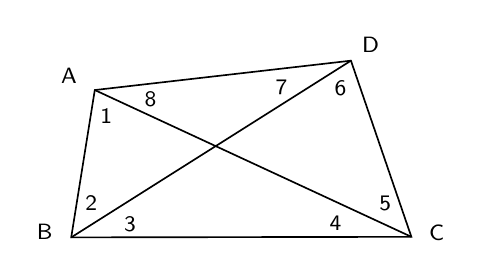
\begin{tikzpicture}[x=.72cm,y=.72cm,line width=.6pt,font=\footnotesize\sffamily]
 \coordinate (A) at (.416,2.599);
 \coordinate (B) at (0,0);
 \coordinate (C) at (6,.01);
 \coordinate (D) at (4.934,3.117);
 \draw (A)--(B)--(C)--(D)--cycle;
 \draw (A)--(C) (B)--(D);
 \node at (-.041,2.843) {A};
 \node at (-.467,.091) {B};
 \node at (6.447,.081) {C};
 \node at (5.279,3.401) {D};
 \node at (.619,2.132) {1};
 \node at (.355,.609) {2};
 \node at (1.035,.233) {3};
 \node at (4.66,.253) {4};
 \node at (5.54,.61) {5};
 \node at (4.75,2.63) {6};
 \node at (3.71,2.64) {7};
 \node at (1.40,2.44) {8};
\end{tikzpicture}
\end{center}
\[
\GaussRightBrace{\begin{array}{@{}l@{\;=\;}l@{}}
 \sin1\,.\sin3\,.\sin(6+7)&\sin(2+3)\,.\sin6\,.\sin8\\
 \sin3\,.\sin5\,.\sin(8+1)&\sin(4+5)\,.\sin8\,.\sin2\\
 \sin5\,.\sin7\,.\sin(2+3)&\sin(6+7)\,.\sin2\,.\sin4\\
 \sin7\,.\sin1\,.\sin(4+5)&\sin(8+1)\,.\sin4\,.\sin6.
\end{array}}\quad\text{\tikz[baseline=-.55ex,x=1mm,y=1mm,line width=.4pt]{\draw (0,1.2)--(-1.25,-.6)--(1.25,-.6)--cycle;\draw (0,-1.2)--(-1.25,.6)--(1.25,.6)--cycle;}}
\]

Am günstigsten ist es, die \(1.,2.,3.\) oder \(4.\) Form zu verwenden, je nachdem, welches der Dreiecke \(ABD,ABC,BCD,ACD\) das größte ist.

Mir ist nicht ganz klar, wie Sie sich vorgestellt haben, \raisebox{.8ex}{.}\,eine gemessene Diagonalrichtung zu verwenden\textsuperscript{[*)]}. Daraus folgt ja, dass, wenn sechs Größen \(A,B,C,D,E,F\) gemessen worden wären, zwischen ihren Korrekturen die Bedingungsgleichung
\[
 \partial A-\partial B+\partial C-\partial D+\partial E-\partial F=\text{Gegebene Größe}
\]

\par\noindent\rule{4cm}{.4pt}\par
{\footnotesize\noindent\hspace*{\parindent}[*) \textsc{Gerling} glaubte, noch zwei Winkelgleichungen mit jeweils null als konstantem Glied aufstellen zu müssen, wenn in einem Viereck die eine Diagonale nur von einem Ende aus beobachtet wurde.]\par}
\noindent{\small IX.}\hfill{\small 32}\hspace*{.12\linewidth}\par

% Printed 250; principal PDF 257; Google PDF 261.
\par\clearpage
\noindent\makebox[0pt][l]{\fontsize{13}{16}\selectfont 250}\hfill{\small\textbf{BRIEFWECHSEL.}}\hfill\null\par\medskip

\noindent gelten würde und nun, weil die sechste, \(F\), \textls[120]{nicht} gemessen wurde, die Bedingungsgleichung
\[
 \partial A-\partial B+\partial C-\partial D+\partial E=0
\]
\noindent gelten müsste. Eine solche Bedingungsgleichung ist jedoch völlig unzulässig, und addiert man die beiden Gleichungen, die Sie anführen, ergibt sich sogar etwas, das in direktem Widerspruch zum Übrigen steht.

Alle Diagonaleinschnitte lassen sich nur mit \textls[120]{denjenigen} Bedingungsgleichungen berücksichtigen, die sich aus Gleichungen wie den oben mit \mbox{\tikz[baseline=-.55ex,x=1mm,y=1mm,line width=.4pt]{\draw (0,1.2)--(-1.25,-.6)--(1.25,-.6)--cycle;\draw (0,-1.2)--(-1.25,.6)--(1.25,.6)--cycle;}} bezeichneten ergeben. Es macht dabei gar keinen Unterschied, ob der Einschnitt auch in Gegenrichtung beobachtet wurde oder nicht. Nur im ersten Fall kommt noch die Bedingungsgleichung hinzu, die aus der Winkelsumme des einen Dreiecks entsteht (die aus dem anderen [Dreieck] ist dann bereits implizit in den übrigen enthalten). Im anderen [Fall] entfällt diese Gleichung.

Im Übrigen wiederhole ich, dass mit der Methode, die ich für meine Messungen bevorzugt habe, alles viel einfacher ausfällt. In meinem eigenen Hauptdreieckssystem gibt es übrigens keine solche Diagonale, die nicht auch in Gegenrichtung gemessen wurde. Die wenigen dieser Art, die an den Grenzen vorkommen, wie Hohehagen—Meisner usw., und verschiedene neue Dreieckspunkte, Syk und Hohenhorn, habe ich gar nicht in das System aufgenommen. Ich habe bisher die gesamte Ausgleichung allein auf die vollständige Messung gestützt, die anderen Punkte jedoch gewissermaßen als Nebenpunkte betrachtet, in Bezug auf die die Lage meiner Hauptpunkte als absolut genau gilt. . . . . . .

\bigskip
{\centering
\textsc{Gauss} an \textsc{Gerling}. \quad Göttingen, 19. Januar 1840.\par}
\medskip

. . . . . . Die Lektüre Ihrer schönen Schrift über Ihre \(\Delta\Delta\) hat mich veranlasst, mich noch einmal etwas in die Sache hineinzudenken, und einige Bemerkungen werden vermutlich für Sie von Interesse sein. Obwohl ich Ihnen vorausgesagt hatte, dass Sie bei der Zickzackbehandlung der Bedingungsgleichungen in zwei Gruppen nur eine langsame Konvergenz erreichen würden, war ich doch etwas verwundert, dass Sie nach einem Ihrer Briefe

% Printed 251; principal PDF 258; Google PDF 262.
\par\clearpage
\noindent\null\hfill{\small\textbf{AUSGLEICHUNG EINFACHER FIGUREN.}}\hfill\makebox[0pt][r]{\fontsize{13}{16}\selectfont 251}\par\medskip

\noindent 15-mal alles durchgerechnet haben (nach dem Buch 13-mal. Ich weiß nicht, wie diese Abweichung zu erklären ist). In meinem eigenen Gradmessungssystem hatte ich etwa 50 Bedingungsgleichungen der zweiten und 12 der dritten Art. Hier war die Konvergenz jedoch sehr schnell, sodass schon die dritte [Rechnung] bis auf \(\frac{1}{1000}''\) stabile Ergebnisse lieferte. Das wäre freilich ohne einen besonderen Kunstgriff nicht möglich gewesen, den Sie, wie mir scheint, \textls[120]{nicht} benutzt haben. Ob ich ihn Ihnen vor 15 Jahren gezeigt habe (in einem Ihrer Briefe beziehen Sie sich auf damalige Mitteilungen), weiß ich nicht. Ich bin aber auch unsicher, ob ich ihn damals schon selbst angewandt hatte. Meine großen Ausgleichungsrechnungen habe ich, glaube ich, Anfang 1826 durchgeführt, ich habe aber nirgends einen Zeitpunkt notiert. Ich will versuchen, Ihnen eine Vorstellung davon zu geben, obwohl eine ausführliche Herleitung eine recht umfangreiche Abhandlung ergeben könnte.

Ich nehme also an, dass die Ausgleichung nach den von den Winkelsummen abhängigen Bedingungsgleichungen schon einmal durchgeführt wurde und man nun zu den Bedingungsgleichungen aus den Seitenverhältnissen übergehen will. Der Kürze halber betrachte ich nur ein Vierpunktsystem \(0\,.\,1\,.\,2\,.\,3\). Ist von den vier \(\Delta\Delta\) \(123\) das größte, so verwenden Sie die Formel \(\frac{01}{02}\,.\,\frac{02}{03}\,.\,\frac{03}{01}=1\) (hier sind \(01\) usw. Seiten, von jetzt an bezeichne ich aber mit \(01\) den \textls[120]{Winkel}, den diese Seite mit der Nulllinie in \(0\) bildet). Jene Gleichung liefert Ihnen \textls[120]{unmittelbar} eine Bedingungsgleichung zwischen \(9\) Korrekturen, denn \(\mathrm{d}01,\mathrm{d}02,\mathrm{d}03\) kommen nicht darin vor. Hätten Sie die Formel \(\frac{10}{12}\,.\,\frac{12}{13}\,.\,\frac{13}{10}=1\) verwendet, so hätten Sie eine Bedingungsgleichung zwischen \textls[120]{9 anderen} Korrekturen erhalten, denn \(\mathrm{d}10,\mathrm{d}12,\mathrm{d}13\) hätten gefehlt. Die beiden Bedingungsgleichungen sind also nicht identisch, doch kann man die eine aus der anderen ableiten, wenn man die zum Viereck gehörenden Bedingungsgleichungen der zweiten Art hinzuzieht. Hier liegt nun ein Fall vor, der häufig vorkommt und in dem ein Rat Anwendung findet, den man nicht genug loben kann. Wenn bei einer Untersuchung die Bestandteile symmetrisch vorliegen und man auf mehr als eine Weise zum Ziel kommen kann, wobei die eine ebenso gut scheint wie die andere und man sich also in der Lage von Buridans Esel befindet, dann soll man \textls[120]{keinen dieser Wege wählen}, sondern einen anderen suchen, auf dem allen Bestandteilen das gleiche Recht zukommt. Darüber lassen sich freilich keine allgemeinen Regeln geben,
\par\smallskip
\noindent\hfill{\small 32\textsuperscript{*}}\hspace*{.12\linewidth}\par
